
%v1
\documentclass{amsart}
\usepackage{amssymb, amsmath, amsfonts, amsthm}
\usepackage{graphics, enumerate, mathrsfs, mathtools,tikz-cd,soul,csquotes}
\usepackage{bm,dsfont}
\usetikzlibrary{positioning,arrows,scopes}
%\usepackage[left=1.25in,
%			right=1.25in,
%			top=1.25in,
%			bottom=1.25in]{geometry}
%\usepackage{fancyhdr}
%\pagestyle{fancy}

% COMMENT OUT FOR FINAL VERSION
\usepackage{showkeys}

% SHOW EQN LABELS ONLY IF REFERENCED
\mathtoolsset{showonlyrefs}

\newtheorem{thm}{Theorem}
\newtheorem*{thm*}{Theorem}
\newtheorem{obs}[thm]{Observation}
\newtheorem{prop}[thm]{Proposition}
\newtheorem{lem}[thm]{Lemma}
\newtheorem{cor}[thm]{Corollary}

\theoremstyle{definition}
\newtheorem{prob}[thm]{Problem}
\newtheorem{dfn}[thm]{Definition}
\newtheorem{eg}[thm]{Example}
\newtheorem{rmk}[thm]{Remark}
\newtheorem{conj}[thm]{Conjecture}

\newcommand{\CC}{\mathbb{C}}
\newcommand{\FF}{\mathbb{F}}
\newcommand{\RR}{\mathbb{R}}
\newcommand{\ZZ}{\mathbb{Z}}
\newcommand{\QQ}{\mathbb{Q}}
\newcommand{\NN}{\mathbb{N}}
\newcommand{\PP}{\mathbb{P}}
\newcommand{\cO}{\mathcal{O}}
\newcommand{\cU}{\mathcal{U}}
\newcommand{\cL}{\mathcal{L}}
\newcommand{\cC}{\mathcal{C}}
\newcommand{\cE}{\mathcal{E}}
% indicator function
\newcommand{\one}{\mathds{1}}
% bold one
\newcommand{\bone}{\mathbf{1}}
\newcommand{\boldmu}{\bm{\mu}}
\newcommand{\bolddelta}{\bm{\delta}}
\newcommand{\boldm}{\mathbf{m}}
\newcommand{\boldn}{\mathbf{n}}

% matrix transpose
\newcommand{\tr}{\intercal}
% sum of cofactors
\DeclareMathOperator{\cof}{cof}
% convex hull of vertex set
\DeclareMathOperator{\conv}{conv}
\DeclareMathOperator{\energy}{\cE}
\DeclareMathOperator{\supp}{supp}
%%%% capacity
\DeclareMathOperator{\Capacity}{\textsc{cap}}
\newcommand{\posCap}{c_{pos}}
\DeclareMathOperator{\argmax}{argmax}
\DeclareMathOperator{\argmin}{argmin}
\DeclareMathOperator{\val}{val}
%topological interior
\DeclareMathOperator{\interior}{int}

\DeclareMathOperator{\rspan}{row.span}
\DeclareMathOperator{\Sym}{Sym}
\DeclareMathOperator{\indeg}{indeg}
%\DeclareMathOperator{\ker}{ker}
\DeclareMathOperator{\coker}{coker}
\DeclareMathOperator{\PL}{PL}
%%% use either \Delta or Div %%%
\DeclareMathOperator{\zspan}{span}
\DeclareMathOperator{\im}{im}
\DeclareMathOperator{\Br}{Brk}
\DeclareMathOperator{\ev}{ev}
\DeclareMathOperator{\vol}{vol}
\DeclareMathOperator{\coeff}{coeff}

% spanning trees
\newcommand{\trees}{\mathcal{F}_1}
\newcommand{\forests}{\mathcal{F}}
\renewcommand{\Re}{\mathrm{Re}}
\newcommand{\dsp}{\displaystyle}
\newcommand{\pderiv}[1]{\frac{\partial}{\partial{#1}}}
\newcommand{\angles}[1]{\langle {#1} \rangle}
\newcommand{\degout}{\deg^o}

% for comments
\newcommand{\note}[1]{{\color{red} \sf $\diamondsuit$  {#1} $\diamondsuit$ }}
\newcommand{\todo}[1]{\note{#1}}
\newcommand{\harry}[1]{{\color{red} \sf $\diamondsuit$  Harry: {#1} $\diamondsuit$ }}

\begin{document}
\title[Tree distance minors]{Minors of tree distance matrices}
\author{Harry Richman}
\author{Farbod Shokrieh}
\author{Chenxi Wu}
\date{v1, \today  \,(Preliminary draft, not for circulation).}
%\thanks{This work was partially supported by ....}


\begin{abstract}
We prove a formula for the determinant of 
the principal minors of
the distance matrix of a weighted tree.
This generalizes a result of Graham and Pollak.
\end{abstract}
\maketitle

%\setcounter{tocdepth}{1}
\tableofcontents

\section{Introduction}

Suppose $G = (V,E)$ is a tree with $n$ vertices.
Let $D$ denote the distance matrix of $G$.
In~\cite{graham-pollak}, Graham and Pollak proved that
\begin{equation}\label{eq:full-det}
\det D = (-1)^{n-1} 2^{n-2} (n-1). 
\end{equation}
This identity is remarkable in that the result does not depend on the tree structure,
beyond the number of vertices.
The identity \eqref{eq:full-det} was motivated by a problem in data communication,
and inspired much further research on distance matrices.
%Self-contained proofs are also given in \cite{du-yeh,yan-yeh}.

The main result of this paper is to generalize \eqref{eq:full-det} by replacing $\det D$ with any of its principal minors.
For a subset $S \subset V(G)$, let $D[S]$ denote the submatrix consisting of the $S$-indexed rows and columns of $D$.
\begin{thm}
\label{thm:main}
Suppose $G$ is a tree with $n$ vertices, 
and distance matrix $D$.
Let $S \subset V(G)$ be a nonempty subset of vertices.
Then
\begin{equation}\label{eq:main}
\det D[S] = (-1)^{|S|-1} 2^{|S|-2} \left( (n-1)\, \kappa(G;S)  - \sum_{\mathcal F_2(G;S)} \left(2 - \degout(F,*)\right)^2  \right),
\end{equation}
where 
%$G/S$ denotes the quotient graph that identifies together vertices in $S$,
$\kappa(G;S)$ is the number of $S$-rooted spanning forests of $G$,
$\forests_2(G;S)$ is the set of $(S,*)$-rooted spanning forests of $G$,
%$k(F,*)$ is defined by
%\begin{equation}
%\label{eq:2-minus-deg}
%k(F,*) 
%%= \sum_{x \in V( F_{*})} {2 - \deg(x)} 
%= 2 - \degout(F,*),
%\end{equation}
and
$\degout(F,*)$ denotes the outdegree of the $*$-component of $F$.
%the number of edges from the $*$-component of $F$ to a different component. 
\end{thm}
For definitions of $(S,*)$-rooted spanning forests and other terminology, see \note{TODO: cite section}.
Note that the quantity $\degout(F,*)$ 
% and $(2-\degout(F,*))^2$ 
satisfies the bounds
\[
1 \leq \degout(F,*) \leq |S|.
\]
%\qquad 0 \leq (2 - \degout(F,*))^2 \leq (2 - |S|)^2 .
%assuming $|S| \geq 3$.
When $S = V$ is the full vertex set, the set of $V$-rooted spanning forests is a singleton, consisting of the vertex set with no edges, 
so $\kappa(G; V) = 1$; and moreover the set $\forests_2(G; V)$ of $(V, *)$-rooted spanning forests is empty. 
Thus \eqref{eq:main} recovers the Graham--Pollak identity \eqref{eq:full-det} when $S = V$.

\subsection{Weighted trees}
%Weighted version:
A weighted version of \eqref{eq:full-det} was proved by Bapat--Kirkland--Neumann~\cite{bapat-kirkland-neumann}.
If $\{\alpha_e : e\in E\}$ is a collection of positive edge weights,  the $\alpha$-distance matrix $D_\alpha$ takes the distance along edge $e$ to be $\alpha_e$; then
\begin{equation}\label{eq:w-full-det}
	\det D_{\alpha} = (-1)^{n-1} 2^{n-2} \sum_{e \in E} \alpha_e \prod_{e \in E} \alpha_e .
\end{equation}
The weighted identity \eqref{eq:w-full-det} reduces to \eqref{eq:full-det} when taking all unit weights, $\alpha_e = 1$.
We also prove the following weighted version of our main theorem.
\begin{thm}
\label{thm:w-main}
Suppose $G = (V,E)$ is a finite, weighted tree with edge weights $\{\alpha_e : e \in E\}$, and corresponding weighted distance matrix $D_\alpha$. For any nonempty subset $S \subset V$, we have
\begin{equation}\label{eq:w-main}
\det D_\alpha[S] = (-1)^{|S|-1} 2^{|S|-2} \left( \sum_{E(G)}\alpha_e \sum_{\trees(G;S)} w(T) - \sum_{\forests_2(G;S)} k(F,{*})^2 w(F) \right).
\end{equation}
where 
$\trees(G;S)$ is the set of $S$-rooted spanning forests of $G$,
$\forests_2(G;S)$ is the set of $(S,*)$-rooted spanning forests of $G$,
$w(T)$ and $w(F)$ denote the $\alpha$-weights of the forests $T$ and $F$,
and 
% $k(F,*)$ is defined as 
\begin{equation}
\label{eq:2-minus-deg}
k(F,*) 
%= \sum_{x \in V( F_{*})} {2 - \deg(x)} 
= 2 - \degout(F,*)
\end{equation}
where $\degout(F, *)$ is the outdegree of the $*$-component of $F$, as above.
\end{thm}

It is worth observing that depending on the chosen subset $S \subset V$, the distances appearing in the submatrix $D[S]$ may ignore a large part of the ambient tree $G$.
We could instead replace $G$ by the subtree consisting of paths between vertices in $S$,
which we call $\conv(S,G)$, the {\em convex hull} of $S \subset G$.
To apply formula \eqref{eq:main} or \eqref{eq:w-main} ``efficiently,''
we should replace $G$ with this convex hull $\conv(S,G)$.
However, the formulas as stated are true even without this replacement due to cancellation of terms.

\begin{cor}
\begin{equation}
\frac{\det D[S]}{\cof D[S]} = \frac12 \left( \sum_{E(G)} \alpha_e - \frac{\sum_{\forests_2(G/S)} w(F) k(F,*)^2}{\sum_{\trees(G/S)} w(T)} \right) .
\end{equation}
\end{cor}

\note{add remark / theorem that det/cof is achieved as result of optimization problem}
We remark that the calculation of $\det D[S]$ is related to the following optimization problem: for $ \boldm \in \RR^S$,
\begin{align*}
\text{optimize:} &\quad D[S] \boldm \\
\text{with constraints:} &\quad \bone^\tr \boldm = 1.
\end{align*}
By the theory of Lagrange multipliers, the solution $\boldm^*$ is the vector satsifying
\[
D[S] \boldm^* = \lambda \bone \qquad\text{for some }\lambda \in \RR,
\]
or equivalently 
$ \boldm^* = \lambda (D[S]^{-1} \bone) $.

\begin{thm}[Monotonicity of principal minor ratios]
Suppose $G = (V,E)$ is a finite, weighted tree with distance matrix $D$.
\begin{enumerate}
\item 
If $S \subset V(G)$ is nonempty,
\begin{equation*}
0 \leq \frac{\det D[S]}{\cof D[S]} \leq \frac12 \sum_{E(G)} \alpha_e .
\end{equation*}

\item 
If $\conv(S,G)$ denotes the subtree of $G$ consisting of all paths between points of $S \subset V(G)$,
\begin{equation*}
 \frac{\det D[S]}{\cof D[S]} \leq \frac12 \sum_{E(\conv(S, G))} \alpha_e .
\end{equation*}

\item 
If $A,B \subset V(G)$
are nonempty subsets with
$A \subset B$,
then
\begin{equation*}
 \frac{\det D[A]}{\cof D[A]}  \leq \frac{\det D[B]}{\cof D[B]}  .
\end{equation*}
\end{enumerate}
\end{thm}

\begin{thm}[Nonsingular minors]
Let $G$ be a finite, weighted tree
with distance matrix $D$,
and let $S \subset V(G)$ be a subset of vertices.
If $|S|\geq 2$ then $\det D[S] \neq 0$.
\end{thm}

\subsection{Previous work} 
A formula for the inverse matrix $D^{-1}$ was found by Graham and Lov\'{a}sz in \cite{graham-lovasz}.

\subsection{Notation}

% $\Gamma$ a compact metric graph

$G$ a finite graph, 
loops and parallel edges allowed,
possibly disconnected

$E(G)$ edge set of $G$

$V(G)$ vertex set of $G$

%$\ell : E(G) \to \RR_{>0}$
%is a length function on edges of $G$

$\kappa(G)$ number of spanning trees of $G$

% $\kappa_2(G)$ number of $2$-forests of $G$

$\trees(G)$ the set of spanning trees of $G$

$\forests_2(G)$ the set of $2$-component forests of $G$

$\trees(G;S)$ the set of $S$-rooted spanning forests of $G$

$\forests_2(G;S)$ the set of $(S,*)$-rooted spanning forests of $G$

% $Meas_{\geq 0}(\Gamma)$ positive Borel measures on $\Gamma$

\section{Graph matrices}

For background on enumeration problems for graphs and trees, see Moon \cite{moon}.

Given a graph $G = (V,E)$, let $L \in \RR^{V \times V}$ denote the {\em Laplacian matrix} of $G$.
If $G$ is a weighted graph with edge weights $\alpha_e  \in \RR_{>0}$ for $e \in E$,
let $L$ denote the weighted Laplacian matrix of $G$.

Given $S \subset V$,
let $L[\overline S]$ denote the matrix obtained from $L$ by removing the rows and columns indexed by $S$.

For any graph $G$, let $\kappa(G)$ denote the number of spanning trees of $G$.
The following theorem is due to Kirchhoff.
For any graph $G$, let $\kappa(G)$ denote the number of spanning trees of $G$.
\begin{thm}[All-minors matrix tree theorem]
\label{thm:matrix-tree}
Let $G = (V,E)$ be a finite graph,
and let $L$ denote the Laplacian matrix of $G$.
Then for any nonempty vertex set $S \subset V(G)$,
\begin{equation}
\det L[\overline S] = \kappa( G / S) .
\end{equation}
\end{thm}
Note that $\kappa(G/S)$ is also the number of $S$-rooted spanning forests of $G$.

The following result is due to Bapat--Siviasubramanian.
\begin{thm}[Distance matrix cofactor sums \cite{bapat-sivasubramanian}]
Given a tree $G$,
let $D$ be the distance matrix of $G$, and $L$ the Laplacian matrix.
Let $S \subset V(G)$ be a nonempty subset of vertices of $G$. 
Then
\begin{equation*}
\cof D[S] = (-2)^{|S|-1} \det L[\overline S] .
\end{equation*}
\end{thm}

\subsection{Distance in trees}

Given an edge $e\in E$ and vertices $v,w \in V$, let 
\begin{equation}
\delta(e; v,w) = \begin{cases}
1 &\text{if } \\
0 &\text{if }.
\end{cases}
\end{equation}

Note that we can express the tree distance $d(v,w)$ as a sum over edges
\begin{equation*}
d(v,w) = \sum_{e \in E(G)} \delta(e; v,w)
\qquad\text{where } \delta(e; v,w) = \begin{cases}
1 &\text{if $e$ lies on $v\sim w$ path}, \\
%\text{if }v,w \text{ are on opposite sides of }e, \\
0 &\text{otherwise}.
\end{cases}
\end{equation*}
\begin{itemize}
\item 
If we fix $v$ and $w$, then $\delta(-;v,w) : E(G) \to \{0,1\}$
is the indicator function for the unique $v~ w$ path in $G$.

\item 
On the other hand if we fix $e$ and $v$,
then the deletion $G\setminus e$ has two connected components,
and $\delta(e;v, -) : V(G) \to \{0,1\}$ 
is the indicator function for the component of $G \setminus e$ not containing $v$.
\end{itemize}


\begin{prop}
\label{prop:distance-sum}
\[ d(v,w) = \sum_{e \in E} \ell(e) \delta(e; v,w) .\]
\end{prop}

\subsection{Tree distance}

For $e\in E$ and $v,w \in V$, let
\begin{equation}
\delta(e;v,w) = \begin{cases}
  1 &\text{if $e$ separates  $v$ from $w$}, \\
  0 &\text{otherwise}.
  \end{cases}
\end{equation}
(Note that $\delta(e; v,v) = 0$ for any $e$ and $v$.)

\subsection{Principal cuts}

Given a tree $G = (V,E)$ and an edge $e \in E$, the edge deletion $G \setminus e$ contains two connected components.
Using the implicit orientation on $e = (e^+,e^-)$,
we let $(G \setminus e)^+$ denote the component that contains endpoint $e^+$, respectively $(G\setminus e)^-$ and endpoint $e^-$.

For any $e \in E$ and $v \in V$,
we let
$(G \setminus e)^{v}$ denote the component of $G\setminus e$ containing $v$,
respectively $(G\setminus e)^{\overline v}$ \note{or $(G\setminus e)^{- v}$} for the component not containing $v$.

\subsection{Outdegree of rooted forest}

Given a rooted forest $F$ in $\forests(G;S)$ and $s \in S$,
let $F(s)$ denote the $s$-component of $F$.
We define the {\em outdegree} $\degout(F,s)$ by
\begin{equation}
\label{eq:outdeg}
	\degout(F,s) = \#\{ e = (a,b) \in E : a \in F(s),\, b \not\in F(s)\}.
\end{equation}
In words, $\degout(F,s)$ is the number of edges which connect the $s$-component of $F$ to a different component.
$$
\#\{ e \in E : e \text{ connects the $s$-component of $F$ to a different component}\}
$$
If $F$ is a forest in $\forests_2(G/S)$, let $\degout(F,*)$ denote the outdegree of the floating component.

\begin{lem}
\label{lem:outdeg-sum}
Suppose $G$ is a tree and $H\subset G$ is a (nonempty) connected subgraph.
Then
\[
  \sum_{v \in V(H)} \left( 2 -  \deg(v) \right) = 2 - \degout(H) .
\]
\end{lem}
\begin{proof}
This is straightforward to check by induction on $|V(H)|$,
with base case $|V(H)| = 1$:
if $H = \{v\}$ consists of a single vertex, then $\degout(H) = \deg(v)$.
%
%Now consider $|V(H)| = n > 1$, and suppose the claim is true for $H'$ when $|V(H')| < n$.
%Since $H$ is a subgraph of a tree, it contains a vertex $v_0$ whose $H$-degree is one.
%Let $H_0 = H \setminus v_0$.
%Using the induction hypothesis, we have
%\begin{align}
% \sum_{v \in V(H)} 2 - \deg(v) &= 2 - \deg(v_0) + \sum_{v \in V(H_0)} 2 - \deg(v) \\
% &= 2 - \deg(v_0) + 2 - \degout(H_0) \\
% &= 2 - \left( \degout(H_0) + \deg(v_0) - 2 \right) .
%\end{align}
%Thus it suffices to show that
%\[ 
%  \degout(H) = \degout(H_0) + \deg(v_0) - 2.
%\]
%This hold because $\degout(H_0) + \deg(v_0)$ overcounts the unique edge joining $v_0$ to $H_0$, by two.
\end{proof}


\subsection{Spanning trees and forests}
A {\em spanning tree} of a graph $G$ is a subgraph which 
is connected, has no cycles,
and contains all vertices of $G$.
A {\em spanning forest} of a graph $G$ is a subgraph which 
has no cycles
and 
contains all vertices of $G$. 

Given a set of vertices $S = \{v_1, v_2, \ldots, v_k\}$,
an {\em $S$-rooted spanning forest} of $G$ 
is a spanning forest which has exactly one vertex $v_i$ in each connected component.
An {\em $(S,*)$-rooted spanning forest} of $G$ is a spanning forest which has $|S|+1$ components, where $|S|$ components each contain one vertex of $S$, and the additional component is disjoint from $S$.
We call the component disjoint from $S$ the ``floating component.''

Let 
$$
\kappa_k(v_1|v_2| \cdots | v_k)
$$
denote the number of $k$-component spanning trees which have a vertex $v_i$ in each component.
If $S = \{v_1,\ldots, v_k\}$,
then $\kappa_k(v_1|\cdots| v_k) = \kappa(G/S)$.



If $u, v, w$ are vertices, then let
$$
\kappa_2(u v | w)
$$
denote the number of two-forests which have $u, v$ in one component and $w$ in the other component.

\begin{eg}
Suppose $G$ is the tree with unit edge lengths shown below.
\[
\begin{tikzpicture}[scale=0.8]
	\coordinate (1) at (0,0);
	\coordinate (A) at (1,0);
	\coordinate (B) at (2,0);
	\coordinate (C) at (3,0);
	\coordinate (D) at (4,0);
	\coordinate (2) at (5,0);
	\coordinate (3) at (2,1);
	
	\foreach \c in {1,2,3,A,B,C,D} {
		\fill (\c) circle (2pt);
	}
	\foreach \c in {1,2,3} {
		\draw (\c) circle (3pt);
	}

	\draw (1) -- (A);
	\draw (A) -- (B);
	\draw (B) -- (3);
	\draw (B) -- (C);
	\draw (C) -- (D);
	\draw (D) -- (2);
	
	\foreach \c/\d in {1/left,2/right,3/right} {
		\node[\d=0.2] at (\c) {$\c$};
	}
\end{tikzpicture}
\]
Let $S$ be the set of three leaf vertices.
Then $\trees(G;S)$ contains $11$ forests,
while $\forests_2(G;S)$ contains $19$ forests.
These are shown in Figures~\ref{fig:1-forests} and \ref{fig:2-forests}, respectively.
\end{eg}

\begin{figure}[h]
\centering
% LABEL 1234
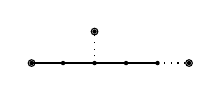
\begin{tikzpicture}[scale=0.4]
	\coordinate (1) at (0,0);
	\coordinate (A) at (1,0);
	\coordinate (B) at (2,0);
	\coordinate (C) at (3,0);
	\coordinate (D) at (4,0);
	\coordinate (2) at (5,0);
	\coordinate (3) at (2,1);
	
	\foreach \c in {1,2,3,A,B,C,D} {
		\fill (\c) circle (2pt);
	}
	\foreach \c in {1,2,3} {
		\draw (\c) circle (3pt);
	}

	\draw (1) -- (A);
	\draw (A) -- (B);
	\draw (B) -- (C);
	\draw (C) -- (D);
	\draw[dotted] (D) -- (2);
	\draw[dotted] (B) -- (3);
\end{tikzpicture}
\qquad
% LABEL 1235
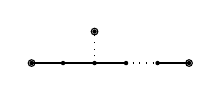
\begin{tikzpicture}[scale=0.4]
	\coordinate (1) at (0,0);
	\coordinate (A) at (1,0);
	\coordinate (B) at (2,0);
	\coordinate (C) at (3,0);
	\coordinate (D) at (4,0);
	\coordinate (2) at (5,0);
	\coordinate (3) at (2,1);
	
	\foreach \c in {1,2,3,A,B,C,D} {
		\fill (\c) circle (2pt);
	}
	\foreach \c in {1,2,3} {
		\draw (\c) circle (3pt);
	}

	\draw (1) -- (A);
	\draw (A) -- (B);
	\draw (B) -- (C);
	\draw[dotted] (C) -- (D);
	\draw (D) -- (2);
	\draw[dotted] (B) -- (3);
\end{tikzpicture}
\qquad
% LABEL 1245
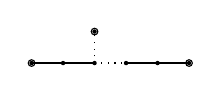
\begin{tikzpicture}[scale=0.4]
	\coordinate (1) at (0,0);
	\coordinate (A) at (1,0);
	\coordinate (B) at (2,0);
	\coordinate (C) at (3,0);
	\coordinate (D) at (4,0);
	\coordinate (2) at (5,0);
	\coordinate (3) at (2,1);
	
	\foreach \c in {1,2,3,A,B,C,D} {
		\fill (\c) circle (2pt);
	}
	\foreach \c in {1,2,3} {
		\draw (\c) circle (3pt);
	}

	\draw (1) -- (A);
	\draw (A) -- (B);
	\draw[dotted] (B) -- (C);
	\draw (C) -- (D);
	\draw (D) -- (2);
	\draw[dotted] (B) -- (3);
\end{tikzpicture}
\\[2em]
% LABEL 1345
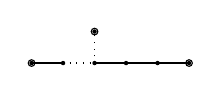
\begin{tikzpicture}[scale=0.4]
	\coordinate (1) at (0,0);
	\coordinate (A) at (1,0);
	\coordinate (B) at (2,0);
	\coordinate (C) at (3,0);
	\coordinate (D) at (4,0);
	\coordinate (2) at (5,0);
	\coordinate (3) at (2,1);
	
	\foreach \c in {1,2,3,A,B,C,D} {
		\fill (\c) circle (2pt);
	}
	\foreach \c in {1,2,3} {
		\draw (\c) circle (3pt);
	}

	\draw (1) -- (A);
	\draw[dotted] (A) -- (B);
	\draw (B) -- (C);
	\draw (C) -- (D);
	\draw (D) -- (2);
	\draw[dotted] (B) -- (3);
\end{tikzpicture}
\qquad
% LABEL 1346
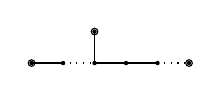
\begin{tikzpicture}[scale=0.4]
	\coordinate (1) at (0,0);
	\coordinate (A) at (1,0);
	\coordinate (B) at (2,0);
	\coordinate (C) at (3,0);
	\coordinate (D) at (4,0);
	\coordinate (2) at (5,0);
	\coordinate (3) at (2,1);
	
	\foreach \c in {1,2,3,A,B,C,D} {
		\fill (\c) circle (2pt);
	}
	\foreach \c in {1,2,3} {
		\draw (\c) circle (3pt);
	}

	\draw (1) -- (A);
	\draw[dotted] (A) -- (B);
	\draw (B) -- (C);
	\draw (C) -- (D);
	\draw[dotted] (D) -- (2);
	\draw (B) -- (3);
\end{tikzpicture}
\qquad
% LABEL 1356
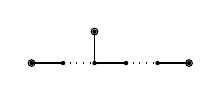
\begin{tikzpicture}[scale=0.4]
	\coordinate (1) at (0,0);
	\coordinate (A) at (1,0);
	\coordinate (B) at (2,0);
	\coordinate (C) at (3,0);
	\coordinate (D) at (4,0);
	\coordinate (2) at (5,0);
	\coordinate (3) at (2,1);
	
	\foreach \c in {1,2,3,A,B,C,D} {
		\fill (\c) circle (2pt);
	}
	\foreach \c in {1,2,3} {
		\draw (\c) circle (3pt);
	}

	\draw (1) -- (A);
	\draw[dotted] (A) -- (B);
	\draw (B) -- (C);
	\draw[dotted] (C) -- (D);
	\draw (D) -- (2);
	\draw (B) -- (3);
\end{tikzpicture}
\qquad
% LABEL 1456
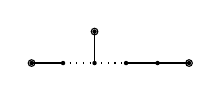
\begin{tikzpicture}[scale=0.4]
	\coordinate (1) at (0,0);
	\coordinate (A) at (1,0);
	\coordinate (B) at (2,0);
	\coordinate (C) at (3,0);
	\coordinate (D) at (4,0);
	\coordinate (2) at (5,0);
	\coordinate (3) at (2,1);
	
	\foreach \c in {1,2,3,A,B,C,D} {
		\fill (\c) circle (2pt);
	}
	\foreach \c in {1,2,3} {
		\draw (\c) circle (3pt);
	}

	\draw (1) -- (A);
	\draw[dotted] (A) -- (B);
	\draw[dotted] (B) -- (C);
	\draw (C) -- (D);
	\draw (D) -- (2);
	\draw (B) -- (3);
\end{tikzpicture}
\\[2em]
% LABEL 2345
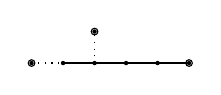
\begin{tikzpicture}[scale=0.4]
	\coordinate (1) at (0,0);
	\coordinate (A) at (1,0);
	\coordinate (B) at (2,0);
	\coordinate (C) at (3,0);
	\coordinate (D) at (4,0);
	\coordinate (2) at (5,0);
	\coordinate (3) at (2,1);
	
	\foreach \c in {1,2,3,A,B,C,D} {
		\fill (\c) circle (2pt);
	}
	\foreach \c in {1,2,3} {
		\draw (\c) circle (3pt);
	}

	\draw[dotted] (1) -- (A);
	\draw (A) -- (B);
	\draw (B) -- (C);
	\draw (C) -- (D);
	\draw (D) -- (2);
	\draw[dotted] (B) -- (3);
\end{tikzpicture}
\qquad
% LABEL 2346
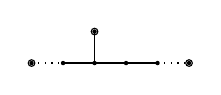
\begin{tikzpicture}[scale=0.4]
	\coordinate (1) at (0,0);
	\coordinate (A) at (1,0);
	\coordinate (B) at (2,0);
	\coordinate (C) at (3,0);
	\coordinate (D) at (4,0);
	\coordinate (2) at (5,0);
	\coordinate (3) at (2,1);
	
	\foreach \c in {1,2,3,A,B,C,D} {
		\fill (\c) circle (2pt);
	}
	\foreach \c in {1,2,3} {
		\draw (\c) circle (3pt);
	}

	\draw[dotted] (1) -- (A);
	\draw (A) -- (B);
	\draw (B) -- (C);
	\draw (C) -- (D);
	\draw[dotted] (D) -- (2);
	\draw (B) -- (3);
\end{tikzpicture}
\qquad
% LABEL 2356
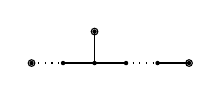
\begin{tikzpicture}[scale=0.4]
	\coordinate (1) at (0,0);
	\coordinate (A) at (1,0);
	\coordinate (B) at (2,0);
	\coordinate (C) at (3,0);
	\coordinate (D) at (4,0);
	\coordinate (2) at (5,0);
	\coordinate (3) at (2,1);
	
	\foreach \c in {1,2,3,A,B,C,D} {
		\fill (\c) circle (2pt);
	}
	\foreach \c in {1,2,3} {
		\draw (\c) circle (3pt);
	}

	\draw[dotted] (1) -- (A);
	\draw (A) -- (B);
	\draw (B) -- (C);
	\draw[dotted] (C) -- (D);
	\draw (D) -- (2);
	\draw (B) -- (3);
\end{tikzpicture}
\qquad
% LABEL 2456
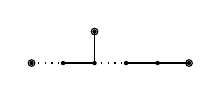
\begin{tikzpicture}[scale=0.4]
	\coordinate (1) at (0,0);
	\coordinate (A) at (1,0);
	\coordinate (B) at (2,0);
	\coordinate (C) at (3,0);
	\coordinate (D) at (4,0);
	\coordinate (2) at (5,0);
	\coordinate (3) at (2,1);
	
	\foreach \c in {1,2,3,A,B,C,D} {
		\fill (\c) circle (2pt);
	}
	\foreach \c in {1,2,3} {
		\draw (\c) circle (3pt);
	}

	\draw[dotted] (1) -- (A);
	\draw (A) -- (B);
	\draw[dotted] (B) -- (C);
	\draw (C) -- (D);
	\draw (D) -- (2);
	\draw (B) -- (3);
\end{tikzpicture}
\caption{Forests in $\trees(G;S)$.}
\label{fig:1-forests}
\end{figure}

\begin{figure}[h]
\centering
% LABEL 123
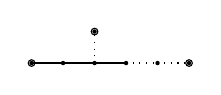
\begin{tikzpicture}[scale=0.4]
	\coordinate (1) at (0,0);
	\coordinate (A) at (1,0);
	\coordinate (B) at (2,0);
	\coordinate (C) at (3,0);
	\coordinate (D) at (4,0);
	\coordinate (2) at (5,0);
	\coordinate (3) at (2,1);
	
	\foreach \c in {1,2,3,A,B,C,D} {
		\fill (\c) circle (2pt);
	}
	\foreach \c in {1,2,3} {
		\draw (\c) circle (3pt);
	}

	\draw (1) -- (A);
	\draw (A) -- (B);
	\draw[dotted] (B) -- (3);
	\draw (B) -- (C);
	\draw[dotted] (C) -- (D);
	\draw[dotted] (D) -- (2);
\end{tikzpicture}
\qquad
% LABEL 124
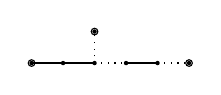
\begin{tikzpicture}[scale=0.4]
	\coordinate (1) at (0,0);
	\coordinate (A) at (1,0);
	\coordinate (B) at (2,0);
	\coordinate (C) at (3,0);
	\coordinate (D) at (4,0);
	\coordinate (2) at (5,0);
	\coordinate (3) at (2,1);
	
	\foreach \c in {1,2,3,A,B,C,D} {
		\fill (\c) circle (2pt);
	}
	\foreach \c in {1,2,3} {
		\draw (\c) circle (3pt);
	}

	\draw (1) -- (A);
	\draw (A) -- (B);
	\draw[dotted] (B) -- (3);
	\draw[dotted] (B) -- (C);
	\draw (C) -- (D);
	\draw[dotted] (D) -- (2);
\end{tikzpicture}
\qquad
% LABEL 125
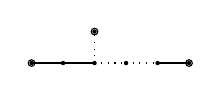
\begin{tikzpicture}[scale=0.4]
	\coordinate (1) at (0,0);
	\coordinate (A) at (1,0);
	\coordinate (B) at (2,0);
	\coordinate (C) at (3,0);
	\coordinate (D) at (4,0);
	\coordinate (2) at (5,0);
	\coordinate (3) at (2,1);
	
	\foreach \c in {1,2,3,A,B,C,D} {
		\fill (\c) circle (2pt);
	}
	\foreach \c in {1,2,3} {
		\draw (\c) circle (3pt);
	}

	\draw (1) -- (A);
	\draw (A) -- (B);
	\draw[dotted] (B) -- (3);
	\draw[dotted] (B) -- (C);
	\draw[dotted] (C) -- (D);
	\draw (D) -- (2);
\end{tikzpicture}
\\[2em]
% LABEL 134
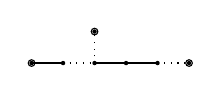
\begin{tikzpicture}[scale=0.4]
	\coordinate (1) at (0,0);
	\coordinate (A) at (1,0);
	\coordinate (B) at (2,0);
	\coordinate (C) at (3,0);
	\coordinate (D) at (4,0);
	\coordinate (2) at (5,0);
	\coordinate (3) at (2,1);
	
	\foreach \c in {1,2,3,A,B,C,D} {
		\fill (\c) circle (2pt);
	}
	\foreach \c in {1,2,3} {
		\draw (\c) circle (3pt);
	}

	\draw (1) -- (A);
	\draw[dotted] (A) -- (B);
	\draw[dotted] (B) -- (3);
	\draw (B) -- (C);
	\draw (C) -- (D);
	\draw[dotted] (D) -- (2);
\end{tikzpicture}
\qquad
% LABEL 135
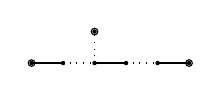
\begin{tikzpicture}[scale=0.4]
	\coordinate (1) at (0,0);
	\coordinate (A) at (1,0);
	\coordinate (B) at (2,0);
	\coordinate (C) at (3,0);
	\coordinate (D) at (4,0);
	\coordinate (2) at (5,0);
	\coordinate (3) at (2,1);
	
	\foreach \c in {1,2,3,A,B,C,D} {
		\fill (\c) circle (2pt);
	}
	\foreach \c in {1,2,3} {
		\draw (\c) circle (3pt);
	}

	\draw (1) -- (A);
	\draw[dotted] (A) -- (B);
	\draw[dotted] (B) -- (3);
	\draw (B) -- (C);
	\draw[dotted] (C) -- (D);
	\draw (D) -- (2);
\end{tikzpicture}
\qquad
% LABEL 136
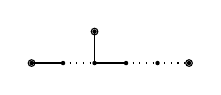
\begin{tikzpicture}[scale=0.4]
	\coordinate (1) at (0,0);
	\coordinate (A) at (1,0);
	\coordinate (B) at (2,0);
	\coordinate (C) at (3,0);
	\coordinate (D) at (4,0);
	\coordinate (2) at (5,0);
	\coordinate (3) at (2,1);
	
	\foreach \c in {1,2,3,A,B,C,D} {
		\fill (\c) circle (2pt);
	}
	\foreach \c in {1,2,3} {
		\draw (\c) circle (3pt);
	}

	\draw (1) -- (A);
	\draw[dotted] (A) -- (B);
	\draw (B) -- (3);
	\draw (B) -- (C);
	\draw[dotted] (C) -- (D);
	\draw[dotted] (D) -- (2);
\end{tikzpicture}
\qquad
% LABEL 145
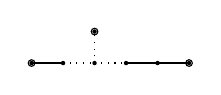
\begin{tikzpicture}[scale=0.4]
	\coordinate (1) at (0,0);
	\coordinate (A) at (1,0);
	\coordinate (B) at (2,0);
	\coordinate (C) at (3,0);
	\coordinate (D) at (4,0);
	\coordinate (2) at (5,0);
	\coordinate (3) at (2,1);
	
	\foreach \c in {1,2,3,A,B,C,D} {
		\fill (\c) circle (2pt);
	}
	\foreach \c in {1,2,3} {
		\draw (\c) circle (3pt);
	}

	\draw (1) -- (A);
	\draw[dotted] (A) -- (B);
	\draw[dotted] (B) -- (3);
	\draw[dotted] (B) -- (C);
	\draw (C) -- (D);
	\draw (D) -- (2);
\end{tikzpicture}
\\[2em]
% LABEL 146
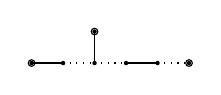
\begin{tikzpicture}[scale=0.4]
	\coordinate (1) at (0,0);
	\coordinate (A) at (1,0);
	\coordinate (B) at (2,0);
	\coordinate (C) at (3,0);
	\coordinate (D) at (4,0);
	\coordinate (2) at (5,0);
	\coordinate (3) at (2,1);
	
	\foreach \c in {1,2,3,A,B,C,D} {
		\fill (\c) circle (2pt);
	}
	\foreach \c in {1,2,3} {
		\draw (\c) circle (3pt);
	}

	\draw (1) -- (A);
	\draw[dotted] (A) -- (B);
	\draw (B) -- (3);
	\draw[dotted] (B) -- (C);
	\draw (C) -- (D);
	\draw[dotted] (D) -- (2);
\end{tikzpicture}
\qquad
% LABEL 156
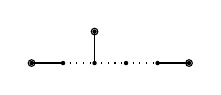
\begin{tikzpicture}[scale=0.4]
	\coordinate (1) at (0,0);
	\coordinate (A) at (1,0);
	\coordinate (B) at (2,0);
	\coordinate (C) at (3,0);
	\coordinate (D) at (4,0);
	\coordinate (2) at (5,0);
	\coordinate (3) at (2,1);
	
	\foreach \c in {1,2,3,A,B,C,D} {
		\fill (\c) circle (2pt);
	}
	\foreach \c in {1,2,3} {
		\draw (\c) circle (3pt);
	}

	\draw (1) -- (A);
	\draw[dotted] (A) -- (B);
	\draw (B) -- (3);
	\draw[dotted] (B) -- (C);
	\draw[dotted] (C) -- (D);
	\draw (D) -- (2);
\end{tikzpicture}
\qquad
% LABEL 234
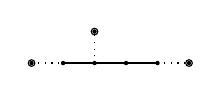
\begin{tikzpicture}[scale=0.4]
	\coordinate (1) at (0,0);
	\coordinate (A) at (1,0);
	\coordinate (B) at (2,0);
	\coordinate (C) at (3,0);
	\coordinate (D) at (4,0);
	\coordinate (2) at (5,0);
	\coordinate (3) at (2,1);
	
	\foreach \c in {1,2,3,A,B,C,D} {
		\fill (\c) circle (2pt);
	}
	\foreach \c in {1,2,3} {
		\draw (\c) circle (3pt);
	}

	\draw[dotted] (1) -- (A);
	\draw (A) -- (B);
	\draw[dotted] (B) -- (3);
	\draw (B) -- (C);
	\draw (C) -- (D);
	\draw[dotted] (D) -- (2);
\end{tikzpicture}
\qquad
% LABEL 235
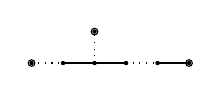
\begin{tikzpicture}[scale=0.4]
	\coordinate (1) at (0,0);
	\coordinate (A) at (1,0);
	\coordinate (B) at (2,0);
	\coordinate (C) at (3,0);
	\coordinate (D) at (4,0);
	\coordinate (2) at (5,0);
	\coordinate (3) at (2,1);
	
	\foreach \c in {1,2,3,A,B,C,D} {
		\fill (\c) circle (2pt);
	}
	\foreach \c in {1,2,3} {
		\draw (\c) circle (3pt);
	}

	\draw[dotted] (1) -- (A);
	\draw (A) -- (B);
	\draw[dotted] (B) -- (3);
	\draw (B) -- (C);
	\draw[dotted] (C) -- (D);
	\draw (D) -- (2);
\end{tikzpicture}
\\[2em]
% LABEL 236
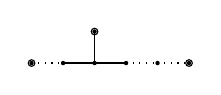
\begin{tikzpicture}[scale=0.4]
	\coordinate (1) at (0,0);
	\coordinate (A) at (1,0);
	\coordinate (B) at (2,0);
	\coordinate (C) at (3,0);
	\coordinate (D) at (4,0);
	\coordinate (2) at (5,0);
	\coordinate (3) at (2,1);
	
	\foreach \c in {1,2,3,A,B,C,D} {
		\fill (\c) circle (2pt);
	}
	\foreach \c in {1,2,3} {
		\draw (\c) circle (3pt);
	}

	\draw[dotted] (1) -- (A);
	\draw (A) -- (B);
	\draw (B) -- (3);
	\draw (B) -- (C);
	\draw[dotted] (C) -- (D);
	\draw[dotted] (D) -- (2);
\end{tikzpicture}
\qquad
% LABEL 245
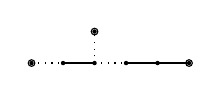
\begin{tikzpicture}[scale=0.4]
	\coordinate (1) at (0,0);
	\coordinate (A) at (1,0);
	\coordinate (B) at (2,0);
	\coordinate (C) at (3,0);
	\coordinate (D) at (4,0);
	\coordinate (2) at (5,0);
	\coordinate (3) at (2,1);
	
	\foreach \c in {1,2,3,A,B,C,D} {
		\fill (\c) circle (2pt);
	}
	\foreach \c in {1,2,3} {
		\draw (\c) circle (3pt);
	}

	\draw[dotted] (1) -- (A);
	\draw (A) -- (B);
	\draw[dotted] (B) -- (3);
	\draw[dotted] (B) -- (C);
	\draw (C) -- (D);
	\draw (D) -- (2);
\end{tikzpicture}
\qquad
% LABEL 246
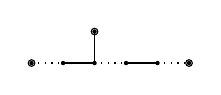
\begin{tikzpicture}[scale=0.4]
	\coordinate (1) at (0,0);
	\coordinate (A) at (1,0);
	\coordinate (B) at (2,0);
	\coordinate (C) at (3,0);
	\coordinate (D) at (4,0);
	\coordinate (2) at (5,0);
	\coordinate (3) at (2,1);
	
	\foreach \c in {1,2,3,A,B,C,D} {
		\fill (\c) circle (2pt);
	}
	\foreach \c in {1,2,3} {
		\draw (\c) circle (3pt);
	}

	\draw[dotted] (1) -- (A);
	\draw (A) -- (B);
	\draw (B) -- (3);
	\draw[dotted] (B) -- (C);
	\draw (C) -- (D);
	\draw[dotted] (D) -- (2);
\end{tikzpicture}
\qquad
% LABEL 256
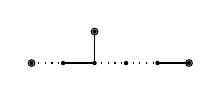
\begin{tikzpicture}[scale=0.4]
	\coordinate (1) at (0,0);
	\coordinate (A) at (1,0);
	\coordinate (B) at (2,0);
	\coordinate (C) at (3,0);
	\coordinate (D) at (4,0);
	\coordinate (2) at (5,0);
	\coordinate (3) at (2,1);
	
	\foreach \c in {1,2,3,A,B,C,D} {
		\fill (\c) circle (2pt);
	}
	\foreach \c in {1,2,3} {
		\draw (\c) circle (3pt);
	}

	\draw[dotted] (1) -- (A);
	\draw (A) -- (B);
	\draw (B) -- (3);
	\draw[dotted] (B) -- (C);
	\draw[dotted] (C) -- (D);
	\draw (D) -- (2);
\end{tikzpicture}
\\[2em]
% LABEL 345
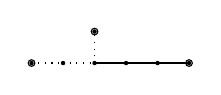
\begin{tikzpicture}[scale=0.4]
	\coordinate (1) at (0,0);
	\coordinate (A) at (1,0);
	\coordinate (B) at (2,0);
	\coordinate (C) at (3,0);
	\coordinate (D) at (4,0);
	\coordinate (2) at (5,0);
	\coordinate (3) at (2,1);
	
	\foreach \c in {1,2,3,A,B,C,D} {
		\fill (\c) circle (2pt);
	}
	\foreach \c in {1,2,3} {
		\draw (\c) circle (3pt);
	}

	\draw[dotted] (1) -- (A);
	\draw[dotted] (A) -- (B);
	\draw[dotted] (B) -- (3);
	\draw (B) -- (C);
	\draw (C) -- (D);
	\draw (D) -- (2);
\end{tikzpicture}
\qquad
% LABEL 346
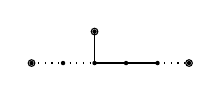
\begin{tikzpicture}[scale=0.4]
	\coordinate (1) at (0,0);
	\coordinate (A) at (1,0);
	\coordinate (B) at (2,0);
	\coordinate (C) at (3,0);
	\coordinate (D) at (4,0);
	\coordinate (2) at (5,0);
	\coordinate (3) at (2,1);
	
	\foreach \c in {1,2,3,A,B,C,D} {
		\fill (\c) circle (2pt);
	}
	\foreach \c in {1,2,3} {
		\draw (\c) circle (3pt);
	}

	\draw[dotted] (1) -- (A);
	\draw[dotted] (A) -- (B);
	\draw (B) -- (3);
	\draw (B) -- (C);
	\draw (C) -- (D);
	\draw[dotted] (D) -- (2);
\end{tikzpicture}
\qquad
% LABEL 356
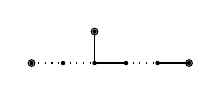
\begin{tikzpicture}[scale=0.4]
	\coordinate (1) at (0,0);
	\coordinate (A) at (1,0);
	\coordinate (B) at (2,0);
	\coordinate (C) at (3,0);
	\coordinate (D) at (4,0);
	\coordinate (2) at (5,0);
	\coordinate (3) at (2,1);
	
	\foreach \c in {1,2,3,A,B,C,D} {
		\fill (\c) circle (2pt);
	}
	\foreach \c in {1,2,3} {
		\draw (\c) circle (3pt);
	}

	\draw[dotted] (1) -- (A);
	\draw[dotted] (A) -- (B);
	\draw (B) -- (3);
	\draw (B) -- (C);
	\draw[dotted] (C) -- (D);
	\draw (D) -- (2);
\end{tikzpicture}
\qquad
% LABEL 456
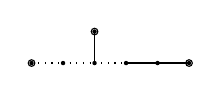
\begin{tikzpicture}[scale=0.4]
	\coordinate (1) at (0,0);
	\coordinate (A) at (1,0);
	\coordinate (B) at (2,0);
	\coordinate (C) at (3,0);
	\coordinate (D) at (4,0);
	\coordinate (2) at (5,0);
	\coordinate (3) at (2,1);
	
	\foreach \c in {1,2,3,A,B,C,D} {
		\fill (\c) circle (2pt);
	}
	\foreach \c in {1,2,3} {
		\draw (\c) circle (3pt);
	}

	\draw[dotted] (1) -- (A);
	\draw[dotted] (A) -- (B);
	\draw (B) -- (3);
	\draw[dotted] (B) -- (C);
	\draw (C) -- (D);
	\draw (D) -- (2);
\end{tikzpicture}
\caption{Forests in $\forests_2(G;S)$.}
\label{fig:2-forests}
\end{figure}


\section{Proofs}
In this section we prove Theorem~\ref{thm:w-main}.

Outline of proof: given a  subset $S \subset V$ and distance submatrix $D[S]$, we will
\begin{enumerate}[(i)]
\item 
Find vector $\mathbf{m} \in \RR^S$ such that $D[S]\mathbf{m} = \lambda \mathbf{1} \in \RR^S$.

\item 
Compute the sum of entries of $\mathbf{m}$, i.e. $\mathbf{1}^\tr \mathbf{m}$.

\item 
Using (i), note the identity
$$ \mathbf{1}^\tr \mathbf{m} 
= \lambda (\mathbf{1}^\tr D[S]^{-1} \mathbf{1}) 
= \lambda \frac{\cof D[S]}{\det D[S]} .$$
where $\cof D[S]$ is the sum of cofactors of $D[S]$.

\item 
Use known expression for $\cof D[S]$ to compute
$$
\det D[S] = \lambda (\cof D[S]) \left( \mathbf{1}^\tr \mathbf{m} \right)^{-1}.
$$
\end{enumerate}
The interesting part  of this expression will turn out to be in the constant $\lambda$.

\begin{eg}
Suppose $G$ is a tree consisting of three paths joined at a central vertex.
Let $S$ consist of the central vertex, and the three endpoints of the paths. 
The corresponding submatrix of the distance matrix is
$$
D[S] = \begin{bmatrix}
0 & a & b & c \\
a & 0 & a + b & a + c \\
b & a + b & 0 & b + c \\
c & a + c & b + c & 0
\end{bmatrix}.
$$
Following the steps outlined above:
\begin{enumerate}[(i)]
\item 
The vector $\mathbf{m} = \begin{bmatrix} -1 \\ 1 \\ 1 \\ 1 \end{bmatrix}$ satisfies
$
D[S] \mathbf{m} = (a+b+c) \mathbf{1}
$

\item 
The sum of entries of $\mathbf{m}$ is $\mathbf{1}^\tr \mathbf{m} = 2$.

\item 
We have 
$$2 = \mathbf{1}^\tr \mathbf{m} = \lambda (\mathbf{1}^\tr D[S]^{-1} \mathbf{1}) = \displaystyle \lambda \frac{\cof D[S]}{\det D[S]}.$$

\item 
The cofactor sum  
$\cof D[S]$ is $-8 abc$,
so the determinant is
\begin{align*}
\det D[S] 
= \lambda \frac{\cof A}{\mathbf{1}^\tr \mathbf{m}}
= (a+b+c) (-8 abc)\frac{1}{2}
= -4(a+b+c)abc.
\end{align*}
\end{enumerate}
\end{eg}

\subsection{Warmup case: $S = V$}

\begin{prop}
Let $G = (V,E)$ a tree, and consider the vector $\mathbf{m} \in \RR^V$
defined by 
\begin{equation}
\mathbf{m}_v = 2 - \deg v
\qquad\text{for each }v\in V.
\end{equation}
% where $\deg v$ denotes the degree of $v$ in $G$.
Then $\mathbf{1}^\tr \mathbf{m} = \sum_{v \in V} (2-\deg v) = 2$.
\end{prop}
\begin{proof}
For any graph, $\sum_{v\in V} \deg v = 2 |E|$.
Since $G$ is a tree, $|E| = |V|-1$.
\end{proof}

\begin{prop}
\label{prop:m-distance-warmup}
Let $\mathbf{m}$ be the vector defined above,
and let $D$ be the distance matrix of $G$.
Then $D \mathbf{m} = \lambda \bone$
for some constant $\lambda$.
\end{prop}
\begin{proof}
%The distance matrix has entries $D_{v,w} = d(v,w)$ which can be expressed as
%\[
%d(v,w) = \sum_{e \in E} \alpha_e \delta(e;v,w),
%\]
%where $\delta(e;v,w)$ is defined in \note{cite}.

%Then for any $w \in V$,
%\begin{align}
%(D \mathbf{m})_w &= \sum_{v \in V} d(v,w) (2 - \deg v) \\
%&= \sum_{v\in V} \left(\sum_{e \in E} \alpha_e \delta(e;v,w)\right) (2 - \deg v) \\
%&= \sum_{e\in E} \alpha_e \left(\sum_{v\in V} \delta(e;v,w) (2 - \deg v) \right) \\
%&= \sum_{e\in E} \alpha_e \sum_{v \in (G\setminus e)^{-w}} (2 - \deg v) \\
%&= \sum_{e\in E} \alpha_e ( 2 - \degout (G\setminus e)^{-w})
%\end{align}
%\note{improve: skip some above details}
It suffices to show that for each edge $e$, with endpoints $(e^+,e^-)$, we have
\[ 
(D \mathbf{m})_{(e^+)} = (D \mathbf{m})_{(e^-)} .
\]
We compute
\begin{align}
(D \mathbf{m})_{(e^+)} - (D \mathbf{m})_{(e^-)} &= \sum_{v \in V} (d(v,e^+) - d(v,e^-)) (2 - \deg v) \\
&= \sum_{v\in (G\setminus e)^-}  \alpha_e (2 - \deg v)  - \sum_{v\in (G\setminus e)^+} \alpha_e (2 - \deg v) 
\label{eq:12-1}
\end{align}
since
\[
d(v,e^+) - d(v,e^-) = \begin{cases}
\alpha_e &\text{if $v$ is closer to $e^-$ than }e^+,\\
- \alpha_e &\text{if $v$ is closer to $e^+$ than }e^-.
\end{cases}
\]
\note{TO DO: define notation $(G \setminus e)^\pm$}
For each sum in \eqref{eq:12-1}, we apply Proposition \note{cite} to obtain
\begin{align}
\alpha_e \sum_{v\in (G\setminus e)^-}  (2 - \deg v)&= \alpha_e (2 - \degout( (G\setminus e)^-) 
= \alpha_e .
\end{align}
The same identity applies to the sum over $(G \setminus e)^+$, so $(D\mathbf{m})_{(e^+)} = (D\mathbf{m})_{(e^-)}$ as desired.
\end{proof}

\subsection{General case: $S \subset V$}
Fix a tree $G = (V,E)$ and a subset $S \subset V$.
\begin{dfn}
\label{dfn:m-vector}
Let $\boldm = \boldm(G;S) \in \RR^S$ be defined by
\begin{equation}
\label{eq:m-vector}
\mathbf{m}_v =  \sum_{T \in \trees(G;S)} 2 - \degout(T,v) 
\qquad\text{for each }v \in S.
\end{equation}
where $\degout(T,v)$ is the outdegree of the $v$-component of $T$, \eqref{eq:outdeg}.
\end{dfn}

Let $\bone$ denote the all-ones vector.
\begin{prop}
For $\boldm$ defined above, $\bone^\tr \boldm = 2 \,\kappa(G;S)$.
\end{prop}
\begin{proof}
We have
\begin{align}
\bone^\tr \boldm = \sum_{s\in S} \boldm_s &= \sum_{s \in S} \left( \sum_{T \in \trees(G;S)} 2 - \degout (T,s) \right) \\
&= \sum_{T \in \trees(G;S)} \left( \sum_{s\in S} \sum_{v \in T(s)} 2 - \deg(v) \right) \\
&= \sum_{T \in \trees(G;S)} \left( \sum_{v \in V} 2 - \deg(v)\right)
= \sum_{T \in \trees(G;S)} 2 .
\end{align}
In the second line we apply Lemma~\ref{lem:outdeg-sum} and exchange the outer summations.
To obtain the third line, we observe that the vertex sets of $T(s)$ for $s \in S$ form a partition of $V$, since $T$ is an $S$-rooted spanning forest. 
Finally we again apply Lemma~\ref{lem:outdeg-sum} for the last equality, as $\degout(G) = 0$.
\end{proof}

\begin{thm}
With $\boldm = \boldm(G;S)$ defined as in \eqref{eq:m-vector},
$D[S] \mathbf{m} = \lambda \mathbf{1}$
for the constant
\begin{equation}
\lambda = \sum_{\trees(G;S)} w(T) \sum_{E(G)} \alpha_e - \sum_{\forests_2(G;S)} w(F) (2 - \degout(F,*) )^2 
\end{equation}
where 
% $k(F,*) = 2 - \degout(F,w)$ and 
$\degout(F,w)$ is the out-degree of the $w$-component of $F$ (as a spanning forest).
\end{thm}
\begin{proof}
For $e\in E$ and $v,w\in V$, let
\[
  \delta(e;v,w) = \begin{cases}
  1 &\text{if $e$ separates  $v$ from $w$}, \\
  0 &\text{otherwise}.
  \end{cases}
\]
For any $v \in S$, we have
\begin{align}
 (D[S] \mathbf{m})_v &= \sum_{s \in S} d(v,s) \mathbf{m}_s \\
 &= \sum_{s \in S} \left( \sum_{e \in E(G)} \alpha_e\, \delta(e; v,s) \right) \left( \sum_{T \in \trees(G;S)} w(T) (2 - \degout(T,s)) \right) \\
 &= \sum_{e\in E} \alpha_e \sum_{T\in \trees } w(T) \sum_{s \in S} (2 - \deg^o(T, s)) \delta(e; v,s) \\
 &= \sum_{e} \alpha_e \sum_{T } w(T) \sum_{s \in S\cap (G\setminus e)^{\overline v}} (2 - \deg^o(T, s)) . \label{eq:14-1}
\end{align}
where
\[ 
S(G\setminus e)^{\overline v} = \{ s \in S : \text{$e$ separates $v$ from $s$}\}
\]
$$
S^*(e,v) = \{ s \in S : \text{$e$ lies on path from $v$ to $s$}\}.
$$
\note{MOVE TO REMARK? If $e \in \conv(G,S)$, then $S(G\backslash e)^{\overline v}$ is nonempty and }
We have
\begin{align*}
\sum_{s \in S(G\setminus e)^{\overline v}}(2 - \degout(T,s)) = \begin{cases}
1 &\text{if }e \not \in T, \\
1 - (2 - \degout(T \setminus e, *)) &\text{if } e \in T(s'),\, s'\in S(G\setminus e)^{\overline v} , \\
1 + (2 - \degout(T \setminus e, *)) &\text{if } e \in T(s'),\, s' \in S(G\setminus e)^v
\end{cases}
\end{align*}
Here 
$T\setminus e$ is a forest in $\forests_2(G;S)$, and
$\degout(T\setminus e, *)$ refers to the out-degree of the ``floating'' component of $T \setminus e$.
These cases correspond to 
\[
(G \setminus e)^{\overline v} = \begin{cases}
\displaystyle
\bigcup_{s \in S(G\setminus e)^{\overline v}} T_s &\text{if } e\not\in T, \\[2em]
\displaystyle
\left( \bigcup_{s \in S(G\setminus e)^{\overline v}} T_s \right) \cup (T\setminus e)_*  &\text{if } e \in T_{s'},\, \delta(e;v,s') = 0 \\[2em]
\displaystyle
\left( \bigcup_{s \in S(G\setminus e)^{\overline v}} T_s \right) \setminus (T\setminus e)_*  &\text{if } e \in T_{s'},\, \delta(e;v,s') = 1 . 
\end{cases}
\]

%If $e \not\in \conv(G,S)$ on the other hand,
%$S^*(e,v)$ is empty and we have
%$$ \sum_{s \in S^*(e,v)} 2 - \deg^o(T,s) = 0 = 1 - (2 - \deg^o(T\setminus e,*))^2,$$
%since $\deg^o(T\setminus e,*) = 1$ in this case. 
From \eqref{eq:14-1} we have
\begin{align*}
(D[S] \mathbf{m})_v &= \sum_{e\in E} \sum_{T\in \trees }  \alpha_e w(T) ( 1 - f(v,e,T) )\\
\end{align*}
where
$$
f(v,e,T) = \begin{cases}
0 &\text{if } e\not\in T\\
2 - \deg^o(T\setminus e,*) &\text{if }  e \in T(s')\text{ for some } s'\in S,\, \delta(e;v,s') = 0 \\
-(2-\deg^o(T\setminus e,*) &\text{if }  e \in T(s')\text{ for some } s'\in S,\, \delta(e;v,s') = 1 \\
\end{cases}
$$
Thus
\begin{align*}
(D[S] \mathbf{m})(v) - \sum_{e \in E} \sum_{T \in \trees}  \alpha_e w(T) 
&= - \sum_{T\in \trees} \sum_{e \in T\setminus T(S^*)} \alpha_e w(T) ( 2 - \deg^o(T\setminus e,*)) \\
&\qquad + \sum_{T \in \trees} \sum_{e  \in T(S^*)} \alpha_e w(T) (2 - \deg^o(T\setminus e,*) )
\end{align*}

If $e \in T$, the deletion $T \setminus e$ is an $(S,*)$-rooted spanning forest of $G$,
so we may rewrite the above expression in terms of $\forests_2(G;S)$.
\begin{align*}
(1) &= - \sum_{F \in \forests_2} w(F) (2 - \deg^o(F,*)) \sum_{T\in \trees} \sum_{e \in T\setminus T(S^*)} \one(F = T \setminus e)  \\
&\qquad +  \sum_{F \in \forests_2} w(F) (2 - \deg^o(F,*)) \sum_{T\in \trees} \sum_{e \in T(S^*)} \one(F = T \setminus e) 
\end{align*}
Next, we note that $F = T \setminus e$ is equivalent to $T = F \cup e$, and in particular this only occurs when we choose $e \in \partial (F,*)$:
\begin{align*}
(1) &= - \sum_{F \in \forests_2} w(F) (2 - \deg^o(F,*))  \sum_{e \in \partial F(*)} \one( \delta(e; v, F(*)) = 1)  \\
&\qquad +  \sum_{F \in \forests_2} w(F) (2 - \deg^o(F,*)) \sum_{e\in \partial F(*)} \one(\delta(e; v, F(*))=0) 
\end{align*}
Here we let $\delta(e; v, F_*)$ denote
\[
\delta(e; v, F_*) = \begin{cases}
0 &\text{if } \\
1 &\text{if }
\end{cases}
\]
Finally, we observe that for any forest $F$ in $\forests_2(G;S)$,
there is exactly one edge $e$ in the boundary $\partial(F, *)$ of the floating component which satisfies $\delta(e; v, F(*)) = 1$, namely the unique boundary edge on the path from $F(*)$ to $v$.
Thus
\[
\#\{e \in \partial F(*) : \delta(e;v, F(*)) = 1 \} = 1
\]
and
\[
\#\{e \in \partial (F,*) : \delta(e;v, F(*)) = 0 \} = \deg^o(F,*) - 1
\]
Thus
\begin{align*}
(1) 
&= - \sum_{F \in \forests_2} w(F) (2 - \deg^o(F,*))  (1)  \\
&\qquad +  \sum_{F \in \forests_2} w(F) (2 - \deg^o(F,*)) (\deg^o(F,*) - 1) \\
&= - \!\!\!\sum_{F \in \forests_2(G/S)} w(F) (2 - \deg^o(F,*))^2 .
\end{align*}
as desired.
\end{proof}

\begin{figure}[h]
% LABEL 1345
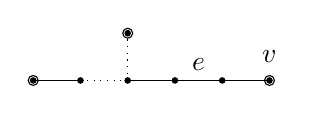
\begin{tikzpicture}[scale=0.6]
	\coordinate (1) at (0,0);
	\coordinate (A) at (1,0);
	\coordinate (B) at (2,0);
	\coordinate (C) at (3,0);
	\coordinate (D) at (4,0);
	\coordinate (2) at (5,0);
	\coordinate (3) at (2,1);
	
	\foreach \c in {1,2,3,A,B,C,D} {
		\fill (\c) circle (2pt);
	}
	\foreach \c in {1,2,3} {
		\draw (\c) circle (3pt);
	}

	\draw (1) -- (A);
	\draw[dotted] (A) -- (B);
	\draw (B) -- (C);
	\draw (C) -- node[above] {$e$} (D);
	\draw (D) -- (2);
	\draw[dotted] (B) -- (3);

	\node[above=0.1] at (2) {$v$};
\end{tikzpicture}
\qquad
% LABEL 1346
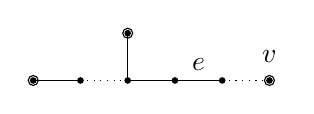
\begin{tikzpicture}[scale=0.6]
	\coordinate (1) at (0,0);
	\coordinate (A) at (1,0);
	\coordinate (B) at (2,0);
	\coordinate (C) at (3,0);
	\coordinate (D) at (4,0);
	\coordinate (2) at (5,0);
	\coordinate (3) at (2,1);
	
	\foreach \c in {1,2,3,A,B,C,D} {
		\fill (\c) circle (2pt);
	}
	\foreach \c in {1,2,3} {
		\draw (\c) circle (3pt);
	}

	\draw (1) -- (A);
	\draw[dotted] (A) -- (B);
	\draw (B) -- (C);
	\draw (C) -- node[above] {$e$} (D);
	\draw[dotted] (D) -- (2);
	\draw (B) -- (3);

	\node[above=0.1] at (2) {$v$};
\end{tikzpicture}
\qquad
% LABEL 1356
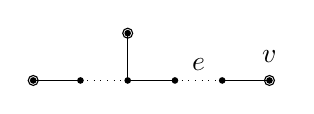
\begin{tikzpicture}[scale=0.6]
	\coordinate (1) at (0,0);
	\coordinate (A) at (1,0);
	\coordinate (B) at (2,0);
	\coordinate (C) at (3,0);
	\coordinate (D) at (4,0);
	\coordinate (2) at (5,0);
	\coordinate (3) at (2,1);
	
	\foreach \c in {1,2,3,A,B,C,D} {
		\fill (\c) circle (2pt);
	}
	\foreach \c in {1,2,3} {
		\draw (\c) circle (3pt);
	}

	\draw (1) -- (A);
	\draw[dotted] (A) -- (B);
	\draw (B) -- (C);
	\draw[dotted] (C) -- node[above] {$e$} (D);
	\draw (D) -- (2);
	\draw (B) -- (3);

	\node[above=0.1] at (2) {$v$};
\end{tikzpicture}
\caption{Components rooted in $S(G\setminus e)^{\overline v}$.}
\end{figure}
 
\begin{figure}[h]
% LABEL 1345
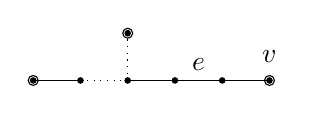
\begin{tikzpicture}[scale=0.6]
	\coordinate (1) at (0,0);
	\coordinate (A) at (1,0);
	\coordinate (B) at (2,0);
	\coordinate (C) at (3,0);
	\coordinate (D) at (4,0);
	\coordinate (2) at (5,0);
	\coordinate (3) at (2,1);
	
	\foreach \c in {1,2,3,A,B,C,D} {
		\fill (\c) circle (2pt);
	}
	\foreach \c in {1,2,3} {
		\draw (\c) circle (3pt);
	}

	\draw (1) -- (A);
	\draw[dotted] (A) -- (B);
	\draw (B) -- (C);
	\draw (C) -- node[above] {$e$} (D);
	\draw (D) -- (2);
	\draw[dotted] (B) -- (3);

	\node[above=0.1] at (2) {$v$};
\end{tikzpicture}
\qquad
% LABEL 1236
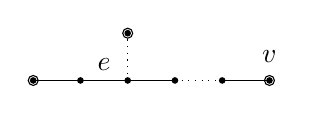
\begin{tikzpicture}[scale=0.6]
	\coordinate (1) at (0,0);
	\coordinate (A) at (1,0);
	\coordinate (B) at (2,0);
	\coordinate (C) at (3,0);
	\coordinate (D) at (4,0);
	\coordinate (2) at (5,0);
	\coordinate (3) at (2,1);
	
	\foreach \c in {1,2,3,A,B,C,D} {
		\fill (\c) circle (2pt);
	}
	\foreach \c in {1,2,3} {
		\draw (\c) circle (3pt);
	}

	\draw (1) -- (A);
	\draw (A) -- node[above] {$e$} (B);
	\draw (B) -- (C);
	\draw[dotted] (C) -- (D);
	\draw (D) -- (2);
	\draw[dotted] (B) -- (3);

	\node[above=0.1] at (2) {$v$};
\end{tikzpicture}
\qquad
% LABEL 1356
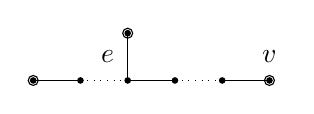
\begin{tikzpicture}[scale=0.6]
	\coordinate (1) at (0,0);
	\coordinate (A) at (1,0);
	\coordinate (B) at (2,0);
	\coordinate (C) at (3,0);
	\coordinate (D) at (4,0);
	\coordinate (2) at (5,0);
	\coordinate (3) at (2,1);
	
	\foreach \c in {1,2,3,A,B,C,D} {
		\fill (\c) circle (2pt);
	}
	\foreach \c in {1,2,3} {
		\draw (\c) circle (3pt);
	}

	\draw (1) -- (A);
	\draw[dotted] (A) -- (B);
	\draw (B) -- (C);
	\draw[dotted] (C) -- (D);
	\draw (D) -- (2);
	\draw (B) -- node[left=0.05] {$e$} (3);

	\node[above=0.1] at (2) {$v$};
\end{tikzpicture}
\caption{Components rooted in $S(G\setminus e)^{\overline v}$.}
\end{figure}

\begin{rmk}
The set $\forests_2(G;S)$ of $(S,*)$-rooted spanning forests of $G$ can be partitioned into two types: ``active'' and ``inactive''.
$$
\forests_2(G/S) = \forests_2^{in}(G/S) \sqcup \forests_2^{out}(G/S),
$$
where
$$
\forests_2^{in}(G/S)  = \{ F \in \forests_2(G/S) \text{ such that } \deg^o(*,F) \geq 2\},
$$
$$
\forests_2^{out}(G/S)  = \{ F \in \forests_2(G/S) \text{ such that } \deg^o(*,F) = 1\}.
$$
\end{rmk}


\begin{rmk}
For a given spanning forest
$F \in \forests_2(G/S, *)$,
there are exactly $\degout(F, *)$ choices of pairs $(T,e) \in \trees(G/S) \times E(G)$ such that
$F = T \setminus e.$
Consider the map
$$
E(G) \times \trees(G/S) \to \forests_2(G/S) \sqcup \{\text{error}\}
$$
defined by ...
$$
(e, T) \mapsto \begin{cases}
T \setminus e &\text{if } e\in T,\\
\text{error} &\text{if } e\not\in T.
\end{cases}
$$
For a forest $F$ in $\forests_2(G/S)$,
the preimage under this map has $\degout(F,*)$ elements.
\end{rmk}

\begin{prop}
Let $G = (V,E)$ be a tree, and $S \subset V$.
Suppose we label $S = \{s_1, \ldots, s_r\}$
and $V \setminus S = \{t_1, \ldots, t_{n-r}\}$.
For each $t_i \in V\setminus S$,
consider
$\mathbf{f}_i  \in \RR^V$
defined by
\end{prop}

\begin{eg}
If 
$$
D[S \cup t] = \begin{bmatrix}
0 & a & b & c \\
a & 0 & a + b & a + c \\
b & a + b & 0 & b + c \\
c & a + c & b + c & 0
\end{bmatrix}
$$
then
$$
 \begin{bmatrix}
0 & a & b & c \\
a & 0 & a + b & a + c \\
b & a + b & 0 & b + c \\
c & a + c & b + c & 0
\end{bmatrix}
\begin{bmatrix}
ab + ac + bc \\ -bc \\ -ac \\ -ab 
\end{bmatrix}
= \begin{bmatrix}
-3abc \\ -abc \\ -abc \\ -abc
\end{bmatrix}
$$
\end{eg}

\section{Physical interpretation}

If we consider $G$ as a network of wires with each edge containing a unit resistor,
which is grounded at all nodes in $S$,
then $\mathbf{m}_S$ records the currents flowing to $S$
when current is added on $V\setminus S$ in the amount $2 - \deg v$
for each $v\not\in S$.

\subsection{Alternate proof}

Let $\mathbf{1}$ denote the all-ones vector.
When we choose a subset $S \subset V(G)$, we no longer have a single ``obvious'' replacement for $\mathbf{m}$ inside $\RR^S$.
Instead, we can take an average over $S$-rooted spanning forests.

In the outline above, our first goal is to find a ``special'' vector $ \mathbf{m}\in \RR^S$ satisfying $D[S] \mathbf{m} = \lambda \mathbf{1}$.
We can approach this first goal as follows: 
consider $\RR^S$ inside the larger vector space $\RR^V = \RR^S \oplus \RR^{V\setminus S}$,
and we wish to find vectors $\mathbf{n}_i \in \RR^{V}$ satisfying
$\pi_S( D \mathbf{n}_i) = \lambda_i \mathbf{1}$.
By finding sufficiently many such vectors $\mathbf{n}_i$,
we can hope to find a linear combination that lies inside $\RR^S \oplus \{0\}$.
% $D \mathbf{n} = (\lambda \mathbf{1}_S) \oplus (-)$.

\begin{prop}
\label{prop:n-vector}
Suppose $v \in V \setminus S$.
For each $s_j \in S$, let $\mu(v,s_j) = $ current flowing to $s_j$
when unit current enters $G$ at $v$ and $G$ is grounded at $S$.
Explicitly,
\begin{equation*}
\mu(v,s) =  \frac{\text{\# of $S$-rooted spanning forests of $G$ whose $s_j$-component contains $v$}}{\text{\# of $S$-rooted spanning forests of $G$}}
% = (\kappa(..))/(\kappa(G/S))
\end{equation*}
\[
= \frac{\sum_{\trees(G/S)} \mathds{1}(v \in T(s))}{\kappa(G/S)}
\]
\[
= \frac{\kappa_{r}(s_1|\cdots|s_j v| \cdots|s_r)}{\kappa_r(s_1|\cdots|s_r)}
\]
Consider the vector $\mathbf{n} = \mathbf{n}(G;S,v) \in \RR^V$ defined by
$$
\mathbf{n}_v = 1,\qquad
\mathbf{n}_s = -\mu(v,s) \text{ if }s \in S, \qquad
\mathbf{n}_w = 0 \text{ if } w \not\in S \cup v
$$
Then $D\mathbf{n}$ is constant on $S$, i.e. $\pi_S( D \mathbf{n}) = \lambda \mathbf{1}$ for some $\lambda$.
\end{prop}
\begin{proof}[Proof sketch]
For any $s, s' \in S$, consider tracking value of $D \mathbf{n}$ along path from $s$ to $s'$. 
The value of $D \mathbf{n}$ changes according to current flow in the corresponding network, i.e. $D \mathbf{n}$ records electrical potential.
By assumption $S$ is grounded, so $D\mathbf{n}$ takes the same value at $s$ and $s'$.
\end{proof}

\begin{thm}
Let $G$ be a tree, $S$ a nonempty subset of vertices,
and $D[S]$ the corresponding submatrix of the distance matrix.
Suppose $\boldm = \boldm(G;S) \in \RR^{S}$ is defined by \eqref{eq:m-vector};
\begin{equation}
\boldm(G;S)_v = \sum_{T \in \trees(G;S)} \sum_{w \in T_v} (2 - \deg w) 
= \sum_{T \in \trees(G;S)} 2 - \degout(T,v) .
\end{equation}
Then $D[S] \mathbf{m} = \lambda \bone$
for some constant $\lambda$.
\end{thm}
\begin{proof}
Note that
\begin{align}
\mathbf{m}(G;S)
&= \kappa(G/S) \left( \sum_{v \in V}(2 - \deg v) {\bolddelta}(v) 
- \sum_{v \in V \setminus S} (2 - \deg v) \mathbf{n}(G;S,v) 
\right) \\
&= \kappa(G;S) \left( \boldm(G;V) - \sum_{v\in V\setminus S} (2 - \deg v) \boldn(G;S,v) \right)
\end{align}
\note{TODO: elaborate on this equation}
From Proposition~\ref{prop:m-distance-warmup} we know that $D \boldm(G;V)$ is constant on $V$,
and from Proposition~\ref{prop:n-vector} we know that $D \boldn(G;S,v)$ is constant on $S$.
Hence by linearity, $D \boldm(G;S)$ is constant on $S$.
\end{proof}



\section{Examples}

\begin{eg}
Suppose $G$ is a tree consisting of three paths joined at a central vertex.
Let $S$ consist of the central vertex, and the three endpoints of the paths. 
The corresponding minor of the distance matrix is
$$
D[S] = \begin{bmatrix}
0 & a & b & c \\
a & 0 & a + b & a + c \\
b & a + b & 0 & b + c \\
c & a + c & b + c & 0
\end{bmatrix}
\sim \begin{bmatrix}
0 & a & b & c \\
a & -a & a  & a \\
b & b & -b & b \\
c & c & c & -c
\end{bmatrix}
\sim \begin{bmatrix}
0 & a & b & c \\
a & -2a & 0 & 0 \\
b & 0 & -2b & 0 \\
c & 0 & 0 & -2c
\end{bmatrix}.
$$
The determinant is
\begin{align*}
\det D[S] 
= -4(a+b+c)abc.
\end{align*}
\end{eg}

\begin{eg}
Suppose $\Gamma$ is a tripod with lengths $a,b,c$ and corresponding leaf vertices $u,v,w$.
\[
\begin{tikzpicture}
	\filldraw[black] (-2,0) coordinate (u) circle (2pt);
	\filldraw[black] (2,1) coordinate (v) circle (2pt);
	\filldraw[black] (2,-1) coordinate (w) circle (2pt);
	\filldraw[black] (0,0) coordinate(o) circle (2pt);

	\draw (o) -- (u);
	\draw (v) -- (o) -- (w);

	\node[left] at (u) {$u$};
	\node[right] at (v) {$v$};
	\node[right] at (w) {$w$};

	\node[above] at (-1,0) {$a$};
	\node[above] at (1,0.5) {$b$};
	\node[below] at (1,-0.5) {$c$};
\end{tikzpicture}
\]
Let $S = \{u,v,w\}$.
Then 
$$
D[S] = \begin{bmatrix}
0 & a + b & a + c \\
a + b & 0 & b + c \\
a + c & b + c & 0
\end{bmatrix}.
$$
and
\begin{align*}
\det D[S] &= 2(a+b)(a+c)(b+c) 
= 2\left( (a+b+c)(ab + ac + bc) - abc \right).
\end{align*}
The ``special vector'' that satisfies $D[S] \mathbf{m} = \lambda \mathbf{1}$ in this example is 
$$
\mathbf{m}^\tr = \begin{bmatrix} a(b + c) & b(a + c) & c(a + b) \end{bmatrix} .
$$
\end{eg}

\begin{eg}
Suppose $\Gamma$ is the tree with unit edge lengths shown below, with five leaf vertices.
\[
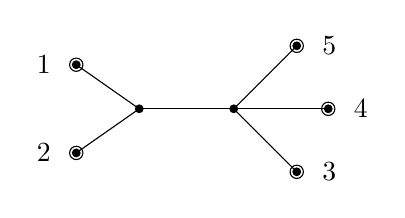
\begin{tikzpicture}[scale=0.8]
	\coordinate (1) at (-2,0.7);
	\coordinate (2) at (-2,-0.7);
	\coordinate (3) at (1.5,-1);
	\coordinate (4) at (2,0);
	\coordinate (5) at (1.5,1);
	\coordinate (A) at (-1,0);
	\coordinate (B) at (0.5,0);
	
	\foreach \c in {1,2,3,4,5,A,B} {
		\fill (\c) circle (2pt);
	}
	\foreach \c in {1,2,3,4,5} {
		\draw (\c) circle (3pt);
	}

	\draw (A) -- (1);
	\draw (A) -- (2);
	\draw (B) -- (3);
	\draw (B) -- (4);
	\draw (B) -- (5);
	\draw (A) -- (B);
	
	\foreach \c/\d in {1/left,2/left,3/right,4/right,5/right} {
		\node[\d=0.2] at (\c) {$\c$};
	}
\end{tikzpicture}
\]
Let $S$ denote the set of five leaf vertices. Then
$$
D[S] = \begin{bmatrix}
0 & 2 & 3 & 3 & 3 \\
2 & 0 & 3 & 3 & 3 \\
3 & 3 & 0 & 2 & 2 \\
3 & 3 & 2 & 0 & 2 \\
3 & 3 & 2 & 2 & 0
\end{bmatrix}.
$$
Forests in $\trees(G;S)$:
\[
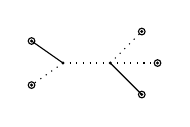
\begin{tikzpicture}[scale=0.4]
	\coordinate (1) at (-2,0.7);
	\coordinate (2) at (-2,-0.7);
	\coordinate (3) at (1.5,-1);
	\coordinate (4) at (2,0);
	\coordinate (5) at (1.5,1);
	\coordinate (A) at (-1,0);
	\coordinate (B) at (0.5,0);
	
	\foreach \c in {1,2,3,4,5,A,B} {
		\fill (\c) circle (1.5pt);
	}
	\foreach \c in {1,2,3,4,5} {
		\draw (\c) circle (3pt);
	}

	\draw (A) -- (1);
	\draw[dotted] (A) -- (2);
	\draw (B) -- (3);
	\draw[dotted] (B) -- (4);
	\draw[dotted] (B) -- (5);
	\draw[dotted] (A) -- (B);
\end{tikzpicture}
\qquad
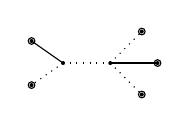
\begin{tikzpicture}[scale=0.4]
	\coordinate (1) at (-2,0.7);
	\coordinate (2) at (-2,-0.7);
	\coordinate (3) at (1.5,-1);
	\coordinate (4) at (2,0);
	\coordinate (5) at (1.5,1);
	\coordinate (A) at (-1,0);
	\coordinate (B) at (0.5,0);
	
	\foreach \c in {1,2,3,4,5,A,B} {
		\fill (\c) circle (1.8pt);
	}
	\foreach \c in {1,2,3,4,5} {
		\draw (\c) circle (3pt);
	}

	\draw (A) -- (1);
	\draw[dotted] (A) -- (2);
	\draw[dotted] (B) -- (3);
	\draw (B) -- (4);
	\draw[dotted] (B) -- (5);
	\draw[dotted] (A) -- (B);
\end{tikzpicture}
\qquad
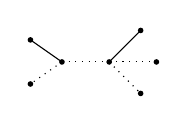
\begin{tikzpicture}[scale=0.4]
	\filldraw[black] (-2,0.7) coordinate (1) circle (2pt);
	\filldraw[black] (-2,-0.7) coordinate (2) circle (2pt);
	\filldraw[black] (1.5,-1) coordinate (3) circle (2pt);
	\filldraw[black] (2,0) coordinate (4) circle (2pt);
	\filldraw[black] (1.5,1) coordinate (5) circle (2pt);
	\filldraw[black] (-1,0) coordinate (A) circle (2pt);
	\filldraw[black] (0.5,0) coordinate (B) circle (2pt);

	\draw (A) -- (1);
	\draw[dotted] (A) -- (2);
	\draw[dotted] (B) -- (3);
	\draw[dotted] (B) -- (4);
	\draw (B) -- (5);
	\draw[dotted] (A) -- (B);
\end{tikzpicture}
\qquad
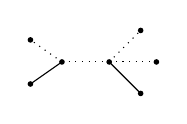
\begin{tikzpicture}[scale=0.4]
	\filldraw[black] (-2,0.7) coordinate (1) circle (2pt);
	\filldraw[black] (-2,-0.7) coordinate (2) circle (2pt);
	\filldraw[black] (1.5,-1) coordinate (3) circle (2pt);
	\filldraw[black] (2,0) coordinate (4) circle (2pt);
	\filldraw[black] (1.5,1) coordinate (5) circle (2pt);
	\filldraw[black] (-1,0) coordinate (A) circle (2pt);
	\filldraw[black] (0.5,0) coordinate (B) circle (2pt);

	\draw[dotted] (A) -- (1);
	\draw (A) -- (2);
	\draw (B) -- (3);
	\draw[dotted] (B) -- (4);
	\draw[dotted] (B) -- (5);
	\draw[dotted] (A) -- (B);
\end{tikzpicture}
\qquad
\begin{tikzpicture}[scale=0.4]
	\filldraw[black] (-2,0.7) coordinate (1) circle (2pt);
	\filldraw[black] (-2,-0.7) coordinate (2) circle (2pt);
	\filldraw[black] (1.5,-1) coordinate (3) circle (2pt);
	\filldraw[black] (2,0) coordinate (4) circle (2pt);
	\filldraw[black] (1.5,1) coordinate (5) circle (2pt);
	\filldraw[black] (-1,0) coordinate (A) circle (2pt);
	\filldraw[black] (0.5,0) coordinate (B) circle (2pt);

	\draw[dotted] (A) -- (1);
	\draw (A) -- (2);
	\draw[dotted] (B) -- (3);
	\draw (B) -- (4);
	\draw[dotted] (B) -- (5);
	\draw[dotted] (A) -- (B);
\end{tikzpicture}
\qquad
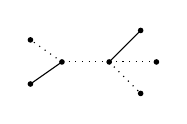
\begin{tikzpicture}[scale=0.4]
	\filldraw[black] (-2,0.7) coordinate (1) circle (2pt);
	\filldraw[black] (-2,-0.7) coordinate (2) circle (2pt);
	\filldraw[black] (1.5,-1) coordinate (3) circle (2pt);
	\filldraw[black] (2,0) coordinate (4) circle (2pt);
	\filldraw[black] (1.5,1) coordinate (5) circle (2pt);
	\filldraw[black] (-1,0) coordinate (A) circle (2pt);
	\filldraw[black] (0.5,0) coordinate (B) circle (2pt);

	\draw[dotted] (A) -- (1);
	\draw (A) -- (2);
	\draw[dotted] (B) -- (3);
	\draw[dotted] (B) -- (4);
	\draw (B) -- (5);
	\draw[dotted] (A) -- (B);
\end{tikzpicture}
\]
\[
\begin{tikzpicture}[scale=0.4]
	\filldraw[black] (-2,0.7) coordinate (1) circle (2pt);
	\filldraw[black] (-2,-0.7) coordinate (2) circle (2pt);
	\filldraw[black] (1.5,-1) coordinate (3) circle (2pt);
	\filldraw[black] (2,0) coordinate (4) circle (2pt);
	\filldraw[black] (1.5,1) coordinate (5) circle (2pt);
	\filldraw[black] (-1,0) coordinate (A) circle (2pt);
	\filldraw[black] (0.5,0) coordinate (B) circle (2pt);

	\draw (A) -- (1);
	\draw[dotted] (A) -- (2);
	\draw[dotted] (B) -- (3);
	\draw[dotted] (B) -- (4);
	\draw[dotted] (B) -- (5);
	\draw (A) -- (B);
\end{tikzpicture}
\qquad
\begin{tikzpicture}[scale=0.4]
	\filldraw[black] (-2,0.7) coordinate (1) circle (2pt);
	\filldraw[black] (-2,-0.7) coordinate (2) circle (2pt);
	\filldraw[black] (1.5,-1) coordinate (3) circle (2pt);
	\filldraw[black] (2,0) coordinate (4) circle (2pt);
	\filldraw[black] (1.5,1) coordinate (5) circle (2pt);
	\filldraw[black] (-1,0) coordinate (A) circle (2pt);
	\filldraw[black] (0.5,0) coordinate (B) circle (2pt);

	\draw[dotted] (A) -- (1);
	\draw (A) -- (2);
	\draw[dotted] (B) -- (3);
	\draw[dotted] (B) -- (4);
	\draw[dotted] (B) -- (5);
	\draw (A) -- (B);
\end{tikzpicture}
\qquad
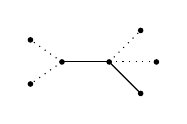
\begin{tikzpicture}[scale=0.4]
	\filldraw[black] (-2,0.7) coordinate (1) circle (2pt);
	\filldraw[black] (-2,-0.7) coordinate (2) circle (2pt);
	\filldraw[black] (1.5,-1) coordinate (3) circle (2pt);
	\filldraw[black] (2,0) coordinate (4) circle (2pt);
	\filldraw[black] (1.5,1) coordinate (5) circle (2pt);
	\filldraw[black] (-1,0) coordinate (A) circle (2pt);
	\filldraw[black] (0.5,0) coordinate (B) circle (2pt);

	\draw[dotted] (A) -- (1);
	\draw[dotted] (A) -- (2);
	\draw (B) -- (3);
	\draw[dotted] (B) -- (4);
	\draw[dotted] (B) -- (5);
	\draw (A) -- (B);
\end{tikzpicture}
\qquad
\begin{tikzpicture}[scale=0.4]
	\filldraw[black] (-2,0.7) coordinate (1) circle (2pt);
	\filldraw[black] (-2,-0.7) coordinate (2) circle (2pt);
	\filldraw[black] (1.5,-1) coordinate (3) circle (2pt);
	\filldraw[black] (2,0) coordinate (4) circle (2pt);
	\filldraw[black] (1.5,1) coordinate (5) circle (2pt);
	\filldraw[black] (-1,0) coordinate (A) circle (2pt);
	\filldraw[black] (0.5,0) coordinate (B) circle (2pt);

	\draw[dotted] (A) -- (1);
	\draw[dotted] (A) -- (2);
	\draw[dotted] (B) -- (3);
	\draw (B) -- (4);
	\draw[dotted] (B) -- (5);
	\draw (A) -- (B);
\end{tikzpicture}
\qquad
\begin{tikzpicture}[scale=0.4]
	\filldraw[black] (-2,0.7) coordinate (1) circle (2pt);
	\filldraw[black] (-2,-0.7) coordinate (2) circle (2pt);
	\filldraw[black] (1.5,-1) coordinate (3) circle (2pt);
	\filldraw[black] (2,0) coordinate (4) circle (2pt);
	\filldraw[black] (1.5,1) coordinate (5) circle (2pt);
	\filldraw[black] (-1,0) coordinate (A) circle (2pt);
	\filldraw[black] (0.5,0) coordinate (B) circle (2pt);

	\draw[dotted] (A) -- (1);
	\draw[dotted] (A) -- (2);
	\draw[dotted] (B) -- (3);
	\draw[dotted] (B) -- (4);
	\draw (B) -- (5);
	\draw (A) -- (B);
\end{tikzpicture}
\]
Forests in $\forests_2(G;S)$:
\[
\begin{tikzpicture}[scale=0.4]
	\coordinate (1) at (-2,0.7);
	\coordinate (2) at (-2,-0.7);
	\coordinate (3) at (1.5,-1);
	\coordinate (4) at (2,0);
	\coordinate (5) at (1.5,1);
	\coordinate (A) at (-1,0);
	\coordinate (B) at (0.5,0);
	
	\foreach \c in {1,2,3,4,5,A,B} {
		\fill (\c) circle (1.5pt);
	}
	\foreach \c in {1,2,3,4,5} {
		\draw (\c) circle (3pt);
	}

	\draw[dotted] (A) -- (1);
	\draw[dotted] (A) -- (2);
	\draw (B) -- (3);
	\draw[dotted] (B) -- (4);
	\draw[dotted] (B) -- (5);
	\draw[dotted] (A) -- (B);
\end{tikzpicture}
\qquad
\begin{tikzpicture}[scale=0.4]
	\coordinate (1) at (-2,0.7);
	\coordinate (2) at (-2,-0.7);
	\coordinate (3) at (1.5,-1);
	\coordinate (4) at (2,0);
	\coordinate (5) at (1.5,1);
	\coordinate (A) at (-1,0);
	\coordinate (B) at (0.5,0);
	
	\foreach \c in {1,2,3,4,5,A,B} {
		\fill (\c) circle (1.5pt);
	}
	\foreach \c in {1,2,3,4,5} {
		\draw (\c) circle (3pt);
	}

	\draw[dotted] (A) -- (1);
	\draw[dotted] (A) -- (2);
	\draw[dotted] (B) -- (3);
	\draw (B) -- (4);
	\draw[dotted] (B) -- (5);
	\draw[dotted] (A) -- (B);
\end{tikzpicture}
\qquad
\begin{tikzpicture}[scale=0.4]
	\coordinate (1) at (-2,0.7);
	\coordinate (2) at (-2,-0.7);
	\coordinate (3) at (1.5,-1);
	\coordinate (4) at (2,0);
	\coordinate (5) at (1.5,1);
	\coordinate (A) at (-1,0);
	\coordinate (B) at (0.5,0);
	
	\foreach \c in {1,2,3,4,5,A,B} {
		\fill (\c) circle (1.5pt);
	}
	\foreach \c in {1,2,3,4,5} {
		\draw (\c) circle (3pt);
	}

	\draw[dotted] (A) -- (1);
	\draw[dotted] (A) -- (2);
	\draw[dotted] (B) -- (3);
	\draw[dotted] (B) -- (4);
	\draw (B) -- (5);
	\draw[dotted] (A) -- (B);
\end{tikzpicture}
\]
\[
\begin{tikzpicture}[scale=0.4]
	\coordinate (1) at (-2,0.7);
	\coordinate (2) at (-2,-0.7);
	\coordinate (3) at (1.5,-1);
	\coordinate (4) at (2,0);
	\coordinate (5) at (1.5,1);
	\coordinate (A) at (-1,0);
	\coordinate (B) at (0.5,0);
	
	\foreach \c in {1,2,3,4,5,A,B} {
		\fill (\c) circle (1.5pt);
	}
	\foreach \c in {1,2,3,4,5} {
		\draw (\c) circle (3pt);
	}

	\draw (A) -- (1);
	\draw[dotted] (A) -- (2);
	\draw[dotted] (B) -- (3);
	\draw[dotted] (B) -- (4);
	\draw[dotted] (B) -- (5);
	\draw[dotted] (A) -- (B);
\end{tikzpicture}
\qquad
\begin{tikzpicture}[scale=0.4]
	\coordinate (1) at (-2,0.7);
	\coordinate (2) at (-2,-0.7);
	\coordinate (3) at (1.5,-1);
	\coordinate (4) at (2,0);
	\coordinate (5) at (1.5,1);
	\coordinate (A) at (-1,0);
	\coordinate (B) at (0.5,0);
	
	\foreach \c in {1,2,3,4,5,A,B} {
		\fill (\c) circle (1.5pt);
	}
	\foreach \c in {1,2,3,4,5} {
		\draw (\c) circle (3pt);
	}

	\draw[dotted] (A) -- (1);
	\draw (A) -- (2);
	\draw[dotted] (B) -- (3);
	\draw[dotted] (B) -- (4);
	\draw[dotted] (B) -- (5);
	\draw[dotted] (A) -- (B);
\end{tikzpicture}
\qquad
\begin{tikzpicture}[scale=0.4]
	\coordinate (1) at (-2,0.7);
	\coordinate (2) at (-2,-0.7);
	\coordinate (3) at (1.5,-1);
	\coordinate (4) at (2,0);
	\coordinate (5) at (1.5,1);
	\coordinate (A) at (-1,0);
	\coordinate (B) at (0.5,0);
	
	\foreach \c in {1,2,3,4,5,A,B} {
		\fill (\c) circle (1.5pt);
	}
	\foreach \c in {1,2,3,4,5} {
		\draw (\c) circle (3pt);
	}

	\draw[dotted] (A) -- (1);
	\draw[dotted] (A) -- (2);
	\draw[dotted] (B) -- (3);
	\draw[dotted] (B) -- (4);
	\draw[dotted] (B) -- (5);
	\draw (A) -- (B);
\end{tikzpicture}
\]
and
$$
\det D[S] = 368
= (-1)^4 2^3 \left( 6 \cdot 11 - (3 \cdot 1^2 + 2 \cdot 2^2 + 1 \cdot 3^2) \right)
$$
\end{eg}

\begin{eg}
Suppose $\Gamma$ is the tree with unit edge lengths shown below, with five leaf vertices and three internal vertices.
\[
\begin{tikzpicture}
	\filldraw[black] (-2,1) coordinate (1) circle (2pt);
	\filldraw[black] (-2,-1) coordinate (2) circle (2pt);
	\filldraw[black] (0,-1) coordinate (3) circle (2pt);
	\filldraw[black] (2,-1) coordinate (4) circle (2pt);
	\filldraw[black] (2,1) coordinate (5) circle (2pt);
	\filldraw[black] (-1,0) coordinate (A) circle (2pt);
	\filldraw[black] (0,0) coordinate (B) circle (2pt);
	\filldraw[black] (1,0) coordinate (C) circle (2pt);

	\node[left] at (1) {$1$};
	\node[left] at (2) {$2$};
	\node[left] at (3) {$3$};
	\node[right] at (4) {$4$};
	\node[right] at (5) {$5$};

	\draw (B) -- (A) -- (1);
	\draw (A) -- (2);
	\draw (3) -- (B) -- (C) -- (4);
	\draw (C) -- (5);
\end{tikzpicture}
\]
Let $S$ denote the set of five leaf vertices. Then
$$
D[S] = \begin{bmatrix}
0 & 2 & 3 & 4 & 4 \\
2 & 0 & 3 & 4 & 4 \\
3 & 3 & 0 & 3 & 3 \\
4 & 4 & 3 & 0 & 2 \\
4 & 4 & 3 & 2 & 0
\end{bmatrix}
$$
and
$$
\det D[S] = 864
= (-1)^4 2^3 \left( 7 \cdot 21 - (14 \cdot 1^2 + 4 \cdot 2^2 + 1 \cdot 3^2) \right)
$$
\end{eg}

\section{Further work}

See \cite{richman-shokrieh-wu}.

\section*{Acknowledgements}
The authors would like to thank Ravindra Bapat for helpful discussion.


\bibliography{tree-distance-ref} 
\bibliographystyle{abbrv}

\end{document}
